% \chapauthor{J. P. Balthasar Mueller}
\chapter{Linear Algebra and Multivariable Calculus}

\begin{multicols}{2}[\subsubsection*{Contents of this chapter}]
   \printcontents{}{1}{\setcounter{tocdepth}{2}}
\end{multicols}




\section{Singular Value Decomposition}




% Cholesky Decomposition
\section{Cholesky Decomposition}
\label{sec:cholesky}

The Cholesky Decomposition exists when a matrix is hermitian and positive-definite. It expresses the matrix $\mathbf{A}$ as:

\begin{equation}
\mathbf{A} = \mathbf{L}\mathbf{L^\dagger}
\end{equation}

Where $\mathbf{L}$ is a lower-triangular matrix with positive, real diagonal entries. When $\mathbf{A}$ is real, then so is $\mathbf{L}$. The Cholesky decomposition enables fast solution of a linear system, but it can also be used to create correlated random variables in Monte Carlo simulations. 

\subsubsection{Creating Correlated Random Variables}
Let $\mathbf{u}_t$ be a vector of uncorrelated samples with sandard deviation 1. If the covariance matrix of the system to be simulated is  $\mathbf{\Sigma}$ with Cholesky decomposition $\mathbf{\Sigma} = \mathbf{LL}^\dagger$, then the vector $\mathbf{v}_t = \mathbf{Lu}_t$ has the desired covariance.

\begin{figure}
\centering
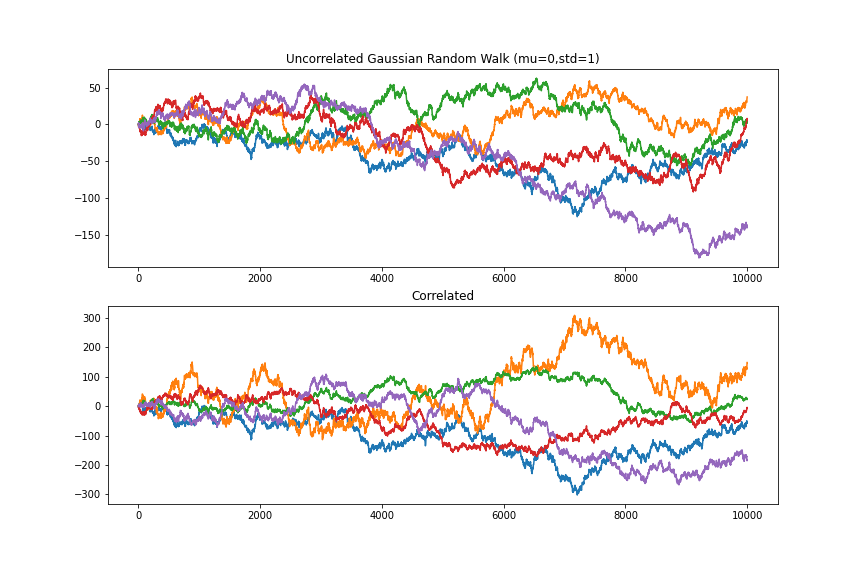
\includegraphics[scale=0.5]{cholesky1.png}
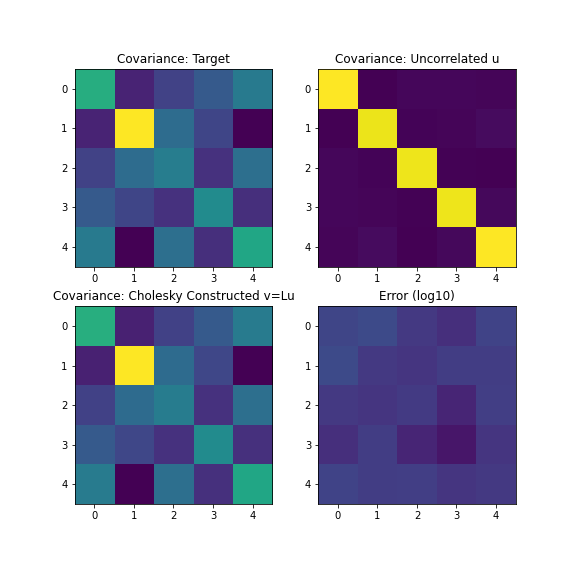
\includegraphics[scale=0.5]{cholesky2.png}
\caption{Creating correlated random variables from uncorrelated random variables using the Cholesky decomposition of the covariance matrix. The 5 uncorrelated random variables are sampled from a standard normal distribution. It is difficult to see a difference between the correlated and uncorrelated random walks.}
\end{figure}

\section{Non-Negative Matrix Factorization}
Non-Negative Matrix Factorization works for positive matrices and is interesting as a method for dimensionality reduction. It works by expressing a matrix $\mathbf{X}\in\mathbb{R}^{p\times n}_+$ in terms of two smaller positive matrices $\mathbf{W}\in\mathbb{R}_+^{p\times r}$ and $\mathbf{H}\in \mathbb{R}^{r\times n}_+$. An excellent introduction is in \possessivecite{morningpaper2019nnmf} blog post and in \citeasnoun{gillis2014and}. 


\section{Generalized Eigenvectors}


\section{$\mathbf{A} = \mathbf{V\Lambda V^{-1}}$ Spectral Theorems, Diagonalization}
\label{sec:diagonalization}

Spectral theorems deal with diagonalizable linear operators. 
\\

A diagonalization of a matrix matrix $\mathbf{A}$ is always possible when a matrix is square, and refers to a decomposition of the matrix into the matrix of eigenvectors $\mathbf{V}$ and eigenvalues $\mathbf{\Lambda}$ as 

\begin{equation}
\mathbf{A} = \mathbf{V\Lambda V^{-1}} 
\end{equation}

\subsection{$\mathbf{A} = \mathbf{V\Lambda V}^T$ Eigendecomposition of Symmetric Matrices}
A symmetric matrix $\mathbf{A}$ has orthogonal eigenvectors so that $\mathbf{V}^{-1} = \mathbf{V}^T$ and real eigenvalues. In that case, the diagonalization is:

\begin{equation}
\mathbf{A} = \mathbf{V\Lambda V}^T = \left[\begin{array}{cccc}
\vrule&\vrule&\hdots&\vrule\\
v_1&v_2&\ddots&v_n\\
\vrule&\vrule&\hdots&\vrule
\end{array}\right]\left[\begin{array}{cccc}
\lambda_1&0&\hdots&0\\ 
0&\lambda_2&\hdots&0\\
\vdots&\vdots&\ddots&\vdots\\
0&\hdots&\hdots&\lambda_n
\end{array}\right]
\left[
\begin{array}{ccc}
\rule[.5ex]{3.5em}{0.4pt}&v_1&\rule[.5ex]{3.5em}{0.4pt}\\
\rule[.5ex]{3.5em}{0.4pt}&v_2&\rule[.5ex]{3.5em}{0.4pt}\\
\vdots&\ddots&\vdots\\
\rule[.5ex]{3.5em}{0.4pt}&v_n&\rule[.5ex]{3.5em}{0.4pt}\\
\end{array}
\right]
\end{equation}

This means that  enables the expression of $\mathbf{A}$ in terms of projections on the eigenvectors:

\begin{equation}
\mathbf{A} = \sum_i \lambda_i (v_i \otimes v_i)
\end{equation}

Where $\otimes$ is the outer product. Since the eigenvectors are an orthonormal basis, $\sum_i v_i \otimes v_i = \mathbb{I}$.


\subsection{$\mathbf{H} = \mathbf{U\Lambda U}^T$ Eigendecomposition of Hermitian Matrices}

Similarly, a hermitian matrix $\mathbf{H} \in \mathbb{C}^{n\times n}$ (the complex equivalent to a symmetric matrix) has real eigenvalues and the matrix of eigenvectors is unitary, so that $\mathbf{H} = \mathbf{U\Lambda U}^T$.


\subsection{Eigenvalue Sensitivity and Accuracy}

\subsubsection{General Case}

In general, the values of the eigenvalues of a square matrix $\mathbf{A}$ may vary wildly under a slight cange of $\mathbf{A} \rightarrow \mathbf{A}+\delta\mathbf{A}$. The sensitivity of the eigenvalues to a change in $\mathbf{A}$ can be investigated using matrix norms \cite{mathworkseig}. Let $||\cdot||$ denote a submultiplicative matrix norm, then:

\begin{equation}
\begin{array}{rl}
\Lambda + \delta\Lambda &= \mathbf{X^{-1}}\left( \mathbf{A} + \delta\mathbf{A} \right)\mathbf{X} \\
\delta\Lambda &= \mathbf{X^{-1}} \delta \mathbf{A} \mathbf{X}\\
||\delta\Lambda || &= ||\mathbf{X^{-1}} \delta \mathbf{A} \mathbf{X} || \leq  ||\mathbf{X^{-1}}|| ||\mathbf{X}|| ||\delta\mathbf{A}||
\end{array}
\end{equation}

When $||\cdot||$ is chosen to be the operator norm with respect to $L^2$, $||\cdot||_{(2)}||$, then $||\mathbf{X^{-1}}|| = \sigma_1$ and $||\mathbf{X}|| = \frac{1}{\sigma_n}$ where $\sigma_1$ and $\sigma_2$ are the square roots of the largest and the smallest eigenvalue of $\mathbf{X^{\dagger}}\mathbf{X}$ respectively (cf. section \ref{sec:norms} on matrix norms). In that case, the sensitivity of the eigenvalues to a change in $\mathbf{A}$ is:

\begin{equation}
||\delta\mathbf{\Lambda}||_{(2)} \leq \frac{\sigma_1}{\sigma_n} ||\delta\mathbf{A}||_{(2)} = \kappa(\mathbf{X})||\delta\mathbf{A}||_{(2)}
\end{equation}

Where $\kappa(\mathbf{X})$ is the conditioning number of the matrix $\mathbf{X}$. Upper bounds on the error on individual eigenvalues can also be derived quite easily, which is shown in \ref{mathworkseig} pp 10-12.

\subsubsection{Hermitian Matrices}
For hermitian (or orthogonal) matrices, the conditioning number for the individual eigenvalues  $\kappa(\lambda_i,\mathbf{H}) = 1$, so that the error on an individual eigenvalue $||\lambda_i||_{(2)} \leq \kappa(\lambda_i,\mathbf{H}) ||\mathbf{H}||_{(2)} = 1\times ||\mathbf{H}||_{(2)}$. 
\section{Types of Transformations}

\subsection{Affine Transformations}

Affine transformations are the combination of a linear map and a translation, which has the form $f(\mathbf{x}) = \mathbf{A}\mathbf{x} + \mathbf{b}$. 

\begin{equation}
f: V \rightarrow W
\end{equation}

Where $V$ and $W$ are vector spaces. Affine transformations can be expresses as matrices by adding an entry with a constant to the vectors that describe a point in space. For example, for $\mathbf{x} \in \mathbb{R}^n$,  the affine transform $f(\mathbf{x}) = \mathbf{A}\mathbf{x} + \mathbf{b}$ with $A\in\mathbb{R}^{n,n}$ and $x,b \in \mathbb{R}^{n}$ can be expressed as the product of a rectangular matrix $\mathbf{M}$ and a vector $\mathbf{c}$ as:

\begin{equation}
\mathbf{A}\mathbf{x} + \mathbf{b} = \underbrace{\left[\begin{array}{c|c} \mathbf{A} & \mathbf{b} \end{array}\right]}_{\mathbf{M}} \underbrace{\left[\begin{array}{c} \mathbf{x} \\ 1\end{array} \right]}_{\mathbf{c}}
\end{equation}

Where $\mathbf{c}^T = \left[x_1,x_2,x_3,...,x_n,1\right]$ and $\mathbf{M} \in \mathbb{R}^{n,n+1}$.

\subsection{Multilinear Maps}

A multilinear map acts on several vectors in a way that is linear in each of its arguments. A $k$-linear map acts on $k$ vectors, where $k=2$ are bilinear maps and $k=1$ are linear maps.

\begin{equation}	
f: V_1 \times V_2 \times ... \times V_n \rightarrow W
\end{equation}

Where $V_1, V_2, ... , V_n$ and $W$ are vector spaces. An example would be the addition or subtraction of two or more vectors.

\subsection{Multilinear Forms}
Multilinear forms are multilinear maps that have a scalar output. An example is the dot product between two vectors, or summing over the elements of one or more vectors.

\begin{equation}
f: V_1 \times V_2 \times ... \times V_n \rightarrow K
\end{equation}

Where $V_1, V_2, ... , V_n$ and $K$ is a scalar field.


\section{Types of Matrices, Matrix Properties}

\subsection{$\mathrm{sgn}\left(\mathbf{x}^{\dagger}\mathbf{H}\mathbf{x}\right)$ Definite}
\label{sec:definite}

A hermitian matrix $\mathbf{H}\in\mathbb{C}^n$ is positive definite, if for any non-zero column vector $\mathbf{x}\in\mathbb{C}^n$, the quadratic form $\mathbf{x}^{\dagger}\mathbf{H}\mathbf{x} > 0$, and negative definite if $\mathbf{x}^{\dagger}\mathbf{H}\mathbf{x} < 0$. The matrix is positive or negative \textit{semidefinite} if  $\mathbf{x}^{\dagger}\mathbf{H}\mathbf{x} \geq 0$ or $\mathbf{x}^{\dagger}\mathbf{H}\mathbf{x} \leq 0$, respectively. Definiteness plays a role in investigating the convexity of a function by looking at the Hessian (section \ref{sec:hessian}). Sometimes notation with curly comparison symbols are used. The relationship between definiteness and eigenvalues is intuitive:

\begin{tabular}{lll}
$\mathbf{H} \succ 0$ & positive definite & all eigenvalues are positive\\
$\mathbf{H} \prec 0$ & negative definite & all eigenvalues are negative\\
$\mathbf{H} \succeq 0$ & positive semidefinite & all eigenvalues are positive or 0\\
$\mathbf{H} \preceq 0$ & negative semidefinite & all eigenvalues are negative or 0
\centering
\end{tabular}

The curly comparison symbols can mean other stuff though, for example in the context of partially ordered sets (order theory) or comparisons between multidimensional arrays.





% unitary
\subsection{Triangular}
\label{sec:triangular}
A lower triangular matrix is a matrix that has all-zero entries above the diagonal.


\begin{equation}
\mathbf{L} = \left[\begin{array}{cccccc} l_{1,1}&&&&&0\\l_{2,1}&l_{2,2}&&&&\\l_{3,1}&l_{3,2}&\ddots&&&\\  \vdots&\vdots&\ddots&\ddots&&\\ \vdots&\vdots&&\ddots&\ddots&\\  l_{n,1}&l_{n,2}&\hdots&\hdots&l_{n,n-1}&l_{n,n}\end{array}\right]
\end{equation}

Upper triangular matrices are matrices that have all-zero entries below the diagonal.



% commuting 
\subsection{$\mathbf{AB}-\mathbf{BA}=0$ Commuting}
Two matrices commute if $\mathbf{AB}=\mathbf{BA}$, or, equivalently, their \textit{commutator} $[\mathbf{A,B}] = \mathbf{AB}-\mathbf{BA}$ is zero. This means that $\mathbf{A}$ and $\mathbf{B}$ both have to be square. Matrices commute when they have the same eigenspace, i.e. they have the same eigenvectors. This can be seen by considering the diagonal representations of $\mathbf{A}$ and $\mathbf{B}$.

Let $\mathbf{A}$ and $\mathbf{B}$ be two square matrices with the same eigenvectors $\mathbf{V}$, then they can be diagonalized as:

\begin{equation}
\mathbf{A} = \mathbf{V\Lambda_A V^{-1}}\\
\mathbf{B} = \mathbf{V\Lambda_B V^{-1}}
\end{equation}

They commute, because:

\begin{equation}
\mathbf{AB} = \mathbf{V\Lambda_A V^{-1}V\Lambda_B V^{-1}} = \mathbf{V\Lambda_B \Lambda_A V^{-1}} = \mathbf{V\Lambda_B V^{-1}V\Lambda_A V^{-1}} = \mathbf{BA} 
\end{equation}



% anticommuting
\subsection{$\mathbf{AB}+\mathbf{BA}=0$ Anticommuting}
Two matrices anticommute if $\mathbf{AB}=-\mathbf{BA}$, or, equivalently, their \textit{anticommutator} $\{\mathbf{A,B}\} = \mathbf{AB}+\mathbf{BA}$ is zero.


% Hermitian / Symmetric
\subsection{$\mathbf{A}^{\dagger} = \mathbf{A}$ Hermitian, Symmetric}
\label{sec:hermitian}
Hermitian matrices are matrices that are equal to their complex transpose. That is:

\begin{equation}
{\mathbf{A}^{*}}^T = \mathbf{A}^\dagger = \mathbf{A} 
\end{equation}

\subsubsection{Properties}
(There are more)
\begin{itemize}
\item By definition: $\mathbf{A} = \mathbf{A}^\dagger$
\item Diagonal Entries are all real, since $a_{i,i} = a_{i,i}^*$, but not necessarily positive (physics will mislead you there...)
\item Inverse is also hermitian:  $\mathbf{A}^{-1} ={ \mathbf{A}^{-1}}^\dagger$
\item Diagonalizable with real eigenvalues and orthogonal eigenvectors $\in \mathbb{C}^n$.
\end{itemize}


Hermitian matrices with only real entries are called symmetric matrices. In that case $\mathbf{A}^T = \mathbf{A}$.

Hermitian matrices can only have real elements along their diagonal. 



% Skew Hermitian / Skew Symmetric
\subsection{$\mathbf{A}^{\dagger} = -\mathbf{A}$ Skew Hermitian, Skew Symmetric}
Skew Hermitian matrices that are equal to the negative of their complex transpose. That is:

\begin{equation}
{\mathbf{A}^{*}}^T = \mathbf{A}^\dagger = -\mathbf{A} 
\end{equation}

Real matrices that are skew Hermitian are called skew symmetric. In that case:

\begin{equation}
\mathbf{A}^T = -\mathbf{A} 
\end{equation}


Skew Hermitian matrices can only have complex values on their diagonal, and skew symmetric matrices can only have zeros as diagonal elements.




% Involutory
\subsection{$\mathbf{A}\mathbf{A}=\mathbf{I}$ Involutory}
Involutory matrixes are matrices that are their own inverse, so that:

\begin{equation}
\mathbf{A}\mathbf{A}=\mathbf{I}
\end{equation}

Involutory matrices are all square roots of the identity matrix. A famous example are the $2\times 2$ Pauli matrices. 




% Isometric
\subsection{$||\mathbf{A}\mathbf{x}||_{\alpha} = ||\mathbf{x}||_{\alpha}$ Isometric}
\label{sec:isometric}
An isometric transformation with respect to some norm $||\cdot||_{\alpha}$ preserves that norm (it's in the name: iso-metric). The linear case is represented by isometric matrices, which satisfy:

\begin{equation}
||\mathbf{A}\mathbf{x}||_{\alpha} = ||\mathbf{x}||_{\alpha} 
\end{equation}

For some vector $\mathbf{x}$. Isometries are also known as distance-preserving maps. To see this, define the distance between two points $\mathbf{a}$ and $\mathbf{b}$ as $||\mathbf{a} - \mathbf{b}||_{\alpha} = ||\mathbf{x}||_{\alpha}$. Isometries are usually understood be bijective. 

In terms of operator norms, isometries must satisfy $||\mathbf{A}||_{(\alpha)} = 1$ where $||\cdot||_{(\alpha)}$ denotes the operator norm (cf. section \ref{sec:operatornorm}). However, operator norms give the upper bound on the distortion of the input, so a unit operator norm is necessary but not sufficient. 


\subsubsection{Isometries with Respect to $L^2$}
The $L^2$ norm is unique in that the points $\{\mathbf{x}: ||\mathbf{x}||_{2} = 1\}$ lie on a perfect circle, which remains a circle regardless of the orientation of the underlying coordinate system. (A sphere looks the same regardless of angle.) This symmetry is broken for all other norms. Unitary matrices are isometries with respect to $L^2$, though unitarity is not a necessary condition for an isometry.

\subsubsection{Isometries with Respect to $L^1$ and general $L^q\neq L^2$}
Isometries with respect to $L^1$ are relevant because they are permissible transformations of (classical) probability distributions. For example, the transition matrix that describes the flow of probability between the time steps of a Markov Chain has to ensure that the entries of the state space probability still sum to $1$. 

For norms $L^q$ with $q\neq2$, the unit "circle" $\{\mathbf{x}: ||\mathbf{x}||_{q\neq2} = 1\}$ is not perfectly round. Instead the symmetry is broken along the coordinate axes. That means that a rotation of the coordinate axes gives a different unit distance, and so two points $\mathbf{a}$ and $\mathbf{b}$ that are $||\mathbf{a}-\mathbf{b}||_{q\neq2} = 1$ apart in one coordinate system may have a different separation in some other coordinate system. 

In particular, for the $L^1$, or \textit{Manhattan} norm (cf. section \ref{sec:l1norm}), the points $\{\mathbf{x}: ||\mathbf{x}||_{1} = 1\}$ lie on a diamond with axes aligned to the axes of the coordinate system. In Manhattan, reaching a point that is $1$ mile away "as the crow flies", depends on the position of that point with respect to the grid of streets and avenues. When that grid is rotated, the point may be quicker or take longer to reach. 

Since this rules out rotations, the internet tells me that the only linear maps that are isometries for $L^q$ with $q\neq 2$ are signed permutation matrices. That is, matrices that assign $\hat{x}\rightarrow \hat{y}$ or $\hat{z} \rightarrow -\hat{x}$ and so on. 

However, in general, any transformation that maps a point on the $L^q$ unit circle to another point on the $L^q$ unit circle is an isometry with respect to $L^q$, and this class of transformation is more general than signed permutations. The stochastic matrices are an example with respect to $L^1$.

\subsection{Stochastic}

Stochastic matrices are used to describe transitions between states of a Markov chain. The matrices are square and each entry is non-negative and represents a conditional probability of moving from one state to another. The entries along either the row or the column, or both, must sum to 1 according to the requirement of marginalization.

\begin{itemize}
\item Right stochastic has rows that sum to 1, so that $\mathbf{P}\mathbf{1}=\mathbf{1}$. It is applied $\mathbf{\pi}\mathbf{P}$. Column index gives "from", row index gives "to". 
\item Left stochastic has columns that sum to 1, so that $\mathbf{1}\mathbf{P}=\mathbf{1}$. It is applied $\mathbf{P}\mathbf{\pi}$. Row index gives "from", column index gives "to".
\item doubly stochastic has rows and columns that sum to 1. 
\end{itemize}

Products of stochastic matrices are also stochastic matrices. The spectral radius (largest eigenvalue) of a stochastic matrix is always $1$. Since $\mathbf{1}$ is an eigenvector and the left and right eigenvalues of a square matrix are the same, there is at least one stationary state $\mathbf{\pi}\mathbf{P}=\mathbf{\pi}$ (that is, in this case of a right stochastic matrix, a left eigenvector) with eigenvalue $1$. 



% Unitary / Orthogonal
\subsection{$\mathbf{U}^{\dagger} = \mathbf{U}^{-1}$ Unitary, Orthogonal}
\label{sec:unitary}
Unitary matrices satisfy $\mathbf{U}^{\dagger}\mathbf{U} = \mathbf{UU}^{\dagger}=\mathbf{I}$, and they have $det(\mathbf{U}) = 1$. They are diagonalizable and can be expressed as $e^{i\mathbf{H}}$ where $\mathbf{H}$ is a Hermitian matrix.

Unitary matrices that are real are called orthogonal.  Orthogonal matrices satisfy $\mathbf{A}^{-1} = \mathbf{A}^T$. The rows (and columns) of $\mathbf{A}$ are an orthonormal basis in $\mathrm{R}^n$.

Unitary matrices are necessarily invertible, and have determinant $|U|=1$ or $|U|=-1$. They represent \textit{unitary transformations}, which means that they preserve the inner product between two vectors.

The set of $n \times n$ orthogonal matrices is known as the orthogonal group $O(n)$ and the subgroup of orthogonal matrices with determinant $1$ is known as the special orthogonal group $SO(n)$. The elements of $SO(n)$ are rotations, and the elements of $O(n)$ represent translations, reflections or rotations. Similarly, the group of $n \times n$ unitary matrices is the unitary group $U(n)$ and the subgroup of $U(n)$ that has determinant $1$ is the special unitary group $SU(n)$.

Unitary transformations preserve the $L^2$ norm of vectors.


% Similarity
\subsection{$\mathbf{A} = \mathbf{TBT^{-1}}$ Similarity}
\label{sec:similiarity}
Two matrices are said to be similar if they can be related through a similarity transformation  $\mathbf{A} = \mathbf{TBT^{-1}}$ where $\mathbf{T}$ is some nonsingular matrix (cf. section \ref{sec:similaritytrans}). An important example is that square matrices are similar to diagonal matrices, see section \ref{sec:diagonalization}. 
   


\section{Properties of Norms}

\section{$L^p$ Lebesgue Vector Norms}
\label{sec:lpnorms}

Let $p\geq1$ be a real number, then the $p$-norm or $L^p$ norm of a vector $\mathbf{x}\in\mathbb{C}^n$ is defined as:

\begin{equation}
||\mathbf{x}||^p = \left[ \sum^n_i |x_i|^p \right]^{1/p}
\end{equation}

The expression can still be useful for $0<p<1$, but in that case the result is not a proper norm, because it is not subadditive (does not satisfy $f(x+y) \leq f(x) + f(y)$). $p$-norms are closely related to expressions for the generalized mean.


\begin{figure}
\centering
    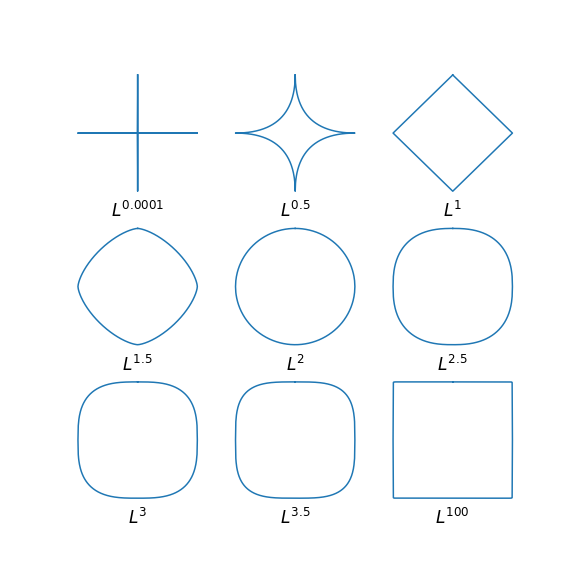
\includegraphics[width=\textwidth]{unitsets.png}
    \caption{Unit Circles: Level sets $\{\mathbf{x}: ||\mathbf{x}||_q = 1\}$ for different $L^q$ norms.}
    \label{fig:svd_eigenfaces}
\end{figure}


\subsection{$L^{1}$ Taxicab / Manhattan Norm}
\label{sec:l1norm}
\begin{equation}
||\mathbf{x}||^1 = \sum_i |x_i|
\end{equation}

In the context of regression, $L^1$ loss gives the maximum likelihood estimator under the assumption of Laplacian (double exponential) distributed errors. For a dataset $\mathbf{x}\in S$, minimizing $\argmin_{\mathbf{s}} \sum_{\mathbf{x}\in S}||\mathbf{x}-\mathbf{s}||_{1}$ gives the median.


\subsection{$L^{2}$ Euclidian Norm}
\label{sec:l2norm}
\begin{equation}
||\mathbf{x}||^2 = \sum_i |x_i|^2
\end{equation}


In the context of regression, $L^2$ loss gives the maximum likelihood estimator under the assumption of normally distributed errors. For a dataset $\mathbf{x}\in S$, minimizing $\argmin_{\mathbf{s}} \sum_{\mathbf{x}\in S}||\mathbf{x}-\mathbf{s}||_{2}$ gives the mean.

I believe that $L^2$ norm should be the only norm that preserves the distance between two points under rotations of the coordinate system.	

\subsection{$L^{\infty}$ Maximum Norm} 

\begin{equation}
||\mathbf{x}||^{\infty} = \max(x_1,x_2,...,x_n)
\end{equation}

For a dataset $\mathbf{x}\in S$, minimizing $\argmin_{\mathbf{s}} \sum_{\mathbf{x}\in S}||\mathbf{x}-\mathbf{s}||_{\infty}$ gives the average of the maximum and the minimum value of the dataset.


\subsection{$L^{-\infty}$ Minimum Norm} 

Formally, I only came across values $0<p$, but it is my opinion that $-\infty$ picks out the minimum value:

\begin{equation}
||\mathbf{x}||^{-\infty} = \min(x_1,x_2,...,x_n)
\end{equation}





\section{Operator and Matrix Norms}
\label{sec:norms}

Matrix norms are functions $||\cdot||: K^{m\times n} \rightarrow \mathbb{R}$ where $K$ is a field of real or complex numbers. They satisfy:

\begin{itemize}
\item $||\alpha A|| = |a| ||A||$ (absolutely homogenous)
\item $||A+B|| \leq ||A|| + ||B||$ (triangle inequality, subadditivity)
\item $||A||\geq 0$ (positive valued)
\item $||A||=0 \implies A_{n,m}=0$ (definiteness)
\end{itemize}

A norm is submultiplicative if it satisfies $||AB||\leq||A||||B||$, which \citeasnoun{rgeraNotes} calls a requirement of "useful matrix norms".

\subparagraph{} 
The main risk of confusion is that norms for operators and vectors are different animals. Norms for operators normally measure some relationship between input and output. Norms for vectors are normally some kind of size, length or distance metric. In as far as matrices can be thought of as both operators and multidimensional vectors, norms of either type may be applied to them. People's notation and language is all over the place. Below I've used $||\cdot||_{(\alpha)}$ to denote norms in the operator sense and $||\cdot||_{\alpha}$ in the vector sense. 

\subsection{$||\mathbf{A}||_{(\alpha)}$ Operator Norm}
\label{sec:operatornorm}
The operator norm describes the largest change in size that it may impart on any of its inputs. That means that the operator norm is defined with respect to a definition of size in both domain and codomain. I.e., for an operator $\mathbf{A}$ and a given way of measuring size $||\cdot||_{\alpha}$:

\begin{equation}
||\mathbf{A}||_{(\alpha)} = \sup\left\{\frac{||\mathbf{A}\mathbf{v}||_{\alpha}}{||\mathbf{x}||_{\alpha}}: \mathbf{v} \in V\right\}
\end{equation}

When the operator is given by a matrix $\mathbf{A}$, and the length of the vector $\mathbf{x}$ is measured using the usual euclidian 2-norm ($||\cdot||_{2}$), then the operator norm is given by the square root of the largest eigenvalue of $\mathbf{A^T A}$. In that case, the operator norm is the same as the 2-norm (cf. section \ref{sec:2norm}).

To re-emphasize, $||A||_{(q)}$ and $||A||_q$ are two different things. The former measures the change in input size, where the size of the input is measured according to the latter. That is the reason for why the 1-Norm and 2-Norms are so different from the vector norms $L_1$ and $L_2$.

Operators that preserve the length of a vector with respect to some norm $||\cdot||_{\alpha}$ satisfy $||\mathbf{A}||_{(\alpha)} = 1$ and are called isometries (cf. section \ref{sec:isometric}). 

% q-norm
\subsection{$||\mathbf{A}||_q$ $q$-Norms}
\label{sec:qnorms}

The $q$ norms for a matrix $\mathbf{A} \in \mathbb{R}^{m\times n}$ with entries $a_{i,j}$ in row $i$ and column $j$ are defined:

\begin{equation}
||\mathbf{A}||_q = \left(\sum_{i}\sum_{j} a^q_{i,j}\right)^{1/q}
\end{equation}

For $q=2$, this becomes the Frobenius norm (section \ref{sec:frobenius}). For vectors $\mathbf{v}\in\mathbb{R}^{n}$, the $q$-norm is more known as $p$-norm or $L^p$ norm (cf. section \ref{sec:lpnorms}). 


% frobenius
\subsection{$||\mathbf{A}||_F$ Frobenius Norm}
\label{sec:frobenius}
The Frobenius Norm is the sum of the squares of all entries of a matrix. Let $\mathbf{A} \in \mathbb{R}^{m\times n}$ be a matrix with entires $a_{i,j}$ in row $i$ and column $j$, then:

\begin{equation}
||\mathbf{A}||_F = \sqrt{\sum_{i}\sum_{j} a^2_{i,j}}
\end{equation}

The Frobenius norm is invariant under rotations, and $||\mathbf{A}||_F = \sqrt{\sum_i \sigma_i^2}$ where $\sigma_i$ are the singular values of $\mathbf{A}$. 

\subsection{$||\mathbf{A}||_{(1)}$ (1)-Norm}
Let $\mathbf{A}$ be a matrix with entires $a_{i,j}$ in row $i$ and column $j$, then:

\begin{equation}
||\mathbf{A}||_{(1)} = \max_{1\leq j \leq n} \sum^m_{i=1} |a_{i,j} |
\end{equation}

That is, it is the maximum of the sums of the absolute values of any of the columns of $\mathbf{A}$.

\subsection{$||\mathbf{A}||_{(\infty)}$ ($\infty$)-Norm}

Let $\mathbf{A}$ be a matrix with entires $a_{i,j}$ in row $i$ and column $j$, then:

\begin{equation}
||\mathbf{A}||_{(\infty)} = \max_{1\leq i \leq m} \sum^n_{j=1} |a_{i,j} |
\end{equation}

That is, it is the maximum of the sums of the absolute values of any of the rows of $\mathbf{A}$.

\subsection{$||\mathbf{A}||_{(2)}$ (2)-Norm}
\label{sec:2norm}

Let $\mathbf{A} \in \mathbb{R}^{m\times n}$ be a matrix with entires $a_{i,j}$ in row $i$ and column $j$, then:

\begin{equation}
||A||_{(2)} = \max_{\mathbf{x}\neq 0} \frac{||\mathbf{Ax}||_2}{||\mathbf{x}||_2}
\end{equation}

Which is the square root of the largest eigenvalue of $A^T A$. Or, equivalently, $||A||_{(2)} = \sigma_1$, where $\sigma_1$ is the largest singular value of the SVD of $\mathbf{A} = \mathbf{U\Sigma V}^T$. That means that $||A^{-1}|| = \frac{1}{\sigma_n}$, where $\sigma_n$ is the smallest singular value of the SVD of $\mathbf{A}$. 





\section{Vector and Matrix Derivatives}
\label{sec:derivatives}

Derivatives involving matrices and vectors can look nonintuitive when the usual symbolic matrix notation is used, but can be derived handily when index notation is used. A very concise and helpful resource for this is \citeasnoun{barnesmatrixdiff}. 


\subsection{Jacobian}
It is particularly helpful to remember the Jacobian, which is the derivative of a function with respect of a vector. The Jacobian of some function $f: \mathbb{R}^n \rightarrow \mathbb{R}^m$ is:

\begin{equation}
\frac{\mathrm{d}  \mathbf{f}(\mathbf{x})}{\mathrm{d} \mathbf{x}}=\left[\frac{\partial \mathbf{f}}{\partial x_1}, \hdots, \frac{\partial \mathbf{f}}{\partial x_n} \right]=\left[\begin{array}{ccc}
\frac{\partial  f_1}{\partial  x_1} & \hdots & \frac{\partial  f_1}{\partial  x_n} \\
\vdots & \vdots & \vdots \\
\frac{\partial  f_m}{\partial  x_1} & \hdots & \frac{\partial  f_m}{\partial  x_n} \\
\end{array}\right]
\end{equation}

I enjoy writing the gradient $\frac{\mathrm{d}}{\mathrm{d}\mathbf{x}}$ as $\nabla_\mathbf{x}$. The relationships below can all be derived as applications of the Jacobian.

\begin{equation}
\begin{array}{l}
\nabla_\mathbf{x} \left(\mathbf{u}^T\mathbf{x}\right) = \left[\frac{\partial }{\partial x_1}\left(\sum_i u_i x_i\right),...,\frac{\partial }{\partial x_n}\left(\sum_i u_i x_i\right)\right] = \mathbf{u}^T\\
\\
\nabla_\mathbf{x} \left(\mathbf{x}^T\mathbf{u}\right) = \left[\frac{\partial }{\partial x_1}\left(\sum_i u_i x_i\right),...,\frac{\partial }{\partial x_n}\left(\sum_i u_i x_i\right)\right] = \mathbf{u}^T\\
\\
\nabla_\mathbf{x} \left(\mathbf{x}^T\mathbf{x}\right) = \left[\frac{\partial }{\partial x_1}\left(\sum_i x_i^2\right),...,\frac{\partial }{\partial x_n}\left(\sum_i x_i^2\right)\right] = 2\mathbf{x}^T\\
\\
\nabla_\mathbf{x} \left(\mathbf{Ax}\right) = \left[
\begin{array}{ccc} 
\underbrace{\frac{\partial }{\partial x_1}\left(\sum_i A_{1i} x_i\right)}_{A_{11}} &...& \underbrace{\frac{\partial }{\partial x_n}\left(\sum_i A_{1i} x_i\right)}_{A_1n}\\
\vdots&\vdots&\vdots\\
\underbrace{\frac{\partial }{\partial x_1}\left(\sum_i A_{ni} x_i\right)}_{A_{n1}} &...& \underbrace{\frac{\partial }{\partial x_n}\left(\sum_i A_{ni} x_i\right)}_{A_{nn}}\\
\end{array}\right] = \mathbf{A}
\end{array}
\end{equation}


\subsection{Inverse Function Theorem}
\label{sec:inverse_function_theorem}
The inverse function theorem gives a sufficient condition for the invertibility of a function near some point in its domain. If the derivative $f'$ of a function $f$ is continuous and non-zero near some point $a$ within its domain, then the function is invertible near that point. If $b = f(a)$, then:

\begin{equation}
\frac{d\left[f^{-1}(b)\right]}{dx} = \frac{1}{\frac{df(a)}{dx}}
\end{equation}

That is, the derivative of the inverse function at a point $b=f(a)$ of the range, is the reciprocal of the derivative of the function near the point $a$ in the domain. This extends to multivariable calculus. Given a function $\mathbf{f}: \mathbf{x} \rightarrow \mathbf{y}$:

\begin{equation}
\nabla_\mathbf{y}\left[\mathbf{f}^{-1}\right] = \left[\nabla_\mathbf{x} \mathbf{f} \right]^{-1}
\end{equation}

In words: the Jacobian of the inverse function at the point $\mathbf{b} = \mathbf{f}(\mathbf{a})$ is the matrix inverse of the Jacobian of the function at the point $\mathbf{a}$. The sufficient condition is that the Jacobian $\nabla_\mathbf{x}\mathbf{f}$ is continuous and \textit{nonsingular} near $\mathbf{a}$.

\subsection{Critical Points}
Critical points are points where the Jacobian does not have maximal rank. In case of a square Jacobian, this means that the Jacobian is singular. 

\subsection{Differential Volume Element, Change of Variables}
The Jacobian is used when transforming between different coordinate systems. Consider a transformation $\mathbf{x} = \mathbf{H}(\mathbf{y})$, then:

\begin{equation}
\mathrm{d}^n x = \left|\nabla_\mathrm{y} \mathbf{H} \right| \mathrm{d}^n y
\end{equation}

And:

\begin{equation}
\int_\mathbf{x} \mathrm{d}^n\mathbf{x} f(\mathbf{x}) = \int_\mathbf{y} \mathrm{d}^n\mathbf{y} \left|\nabla_\mathrm{y} \mathbf{H} \right| f(\mathbf{H}(\mathbf{y}))
\end{equation}

Alternatively, if $\mathbf{y} = \mathbf{H}^{-1}(\mathbf{x})$:

 \begin{equation}
 \begin{array}{rl}
 \mathrm{d}^n y &= \left|\nabla_\mathrm{x} \mathbf{H}^{-1}(\mathbf{x})\right| \mathrm{d}^n x\\
 &= \left| \left[ \nabla_\mathrm{y} \mathbf{H}(\mathbf{y}) \right]^{-1} \right| \mathrm{d}^n x\\
 \mathrm{d}^n x &= \frac{1}{\left| \left[ \nabla_\mathrm{y} \mathbf{H}(\mathbf{y}) \right]^{-1} \right|}  \mathrm{d}^n y 
 \end{array}
 \end{equation}

The Jacobian has to be nonsingular within the domain of integration. This implies that $\mathbf{x}$ and $\mathbf{y}$ have to have the same dimension. In the context of probability theory that sometimes requires artificially defining additional variables so that $\mathbf{H}$ is bijective because the quantity of interest has lower dimension (for example, if you calculate the mean of a random variable). 

\subsection{Hessian}
\label{sec:hessian}

The Hessian is the second derivative of a scalar valued function $f:\mathbb{R}^{n} \rightarrow \mathbb{R}$ with respect to a vector, i.e. $\nabla\cdot\nabla f$. The elements are $\mathbf{H}(f)_{i,j} = \frac{\partial^2 f}{\partial x_i\partial x_j}$. 

\begin{equation}
\mathbf{H}(f) = \left[\begin{array}{cccc}
\frac{\partial^2f}{\partial x_1^2}&\frac{\partial^2f}{\partial x_1\partial x_2} & \hdots & \frac{\partial^2f}{\partial x_1\partial x_n}\\
\frac{\partial^2f}{\partial x_2\partial x_1}&\frac{\partial^2f}{\partial x_2^2} & \hdots & \frac{\partial^2f}{\partial x_1\partial x_n}\\
\vdots & \vdots & \ddots & \vdots \\
\frac{\partial^2f}{\partial x_n\partial x_1}&\frac{\partial^2f}{\partial x_n\partial x_2} & \hdots & \frac{\partial^2f}{\partial x_n^2}
\end{array} \right]
\end{equation}

The Hessian of a vector valued function $f:\mathbb{R}^n \rightarrow \mathbb{R}^m$ is a third order tensor with elements  $\mathbf{H}(\mathbf{f})_{i,j,k} = \frac{\partial^2 f_k}{\partial x_i\partial x_j}$.

\subsubsection{Testing Convexity}
The definiteness (cf. section \ref{sec:definite}) of the Hessian is used to test convexity.

\begin{tabular}{ll}
$\mathbf{H}\succeq 0$ & convex\\
$\mathbf{H}\succ 0$ & strictly convex\\
$\mathbf{H}\preceq 0$ & concave\\
$\mathbf{H}\prec 0$ & strictly concave\\
\end{tabular}

If this holds at a point, the property is local (for example at a local maximum or minimum), and if it holds everywhere on the domain, then the property is global.




\chapauthor{}
